\chapter{Agent training and experiments in ideal simulation environment}
Chapters 4 and 5 focus on the experimental phase of the project. This chapter details the training procedure of SAC agents for the swing-up task and then transitions to a simulation phase in ideal environments to validate results for both the swing-up and stabilization tasks. The chapter is structured into three distinct subsections: training setup, training process, and simulation results.

The first subsection describes the training framework, combining a Stable-Baseline3-based RL algorithm with a customized environment inherited from the OpenAI Gym environment. The second subsection centers on hyperparameter-tuning and highlights the challenges encountered during training. The third subsection displays the results acquired from both the pendubot and acrobot setups in ideal simulations.

\section{Training setup in ideal environment}
Stable Baseline 3(SB3)\cite{stable-baselines3} is an open-source implementation of deep reinforcement learning algorithms based on the Python language. This library includes seven commonly used model-free deep reinforcement learning algorithms including SAC. Prior implementations of deep RL algorithms often encountered a problem wherein small implementation details could greatly affect performance, typically exceeding the differences between algorithms\cite{islam2017reproducibility}. The developers of SB3 have done a commendable job stabilizing the performance of these deep RL algorithms by benchmarking each one on common environments and comparing them to prior implementations. Owing to its user-friendly and reliable nature, we chose Stable Baseline 3 as our RL library, which greatly simplified our research process.

OpenAI Gymnasium\cite{towers_gymnasium_2023} is a toolkit for developing and comparing reinforcement learning algorithms, and it is widely used in the research community. Among its many advantages are its open-source nature and standardized environments, which facilitate the rapid testing and benchmarking of new algorithms. Additionally, it offers easy visualization and monitoring. Our decision to use the Gymnasium library is based on its extensibility—from standard environments to highly customized ones—as well as its capability to integrate with tools like PyTorch and TensorFlow for GPU-accelerated computations. Furthermore, Gymnasium provides the ability to construct stacked training environments for parallel training.

\begin{figure}[htbp]
    \centering
    
\includegraphics[width=0.8\linewidth]{figures/simulation_result/RL_interaction.png}
    \caption{Interaction between reinforcement learning agent and customized environment}
    \label{fig:RL_interaction}
\end{figure}

The construction of the customized environment begins with the dynamic function that captures the nonlinear dynamics of the underactuated double pendulum, as detailed in this repository\cite{2023_ram_wiebe_double_pendulum}. The dynamic function, utilizing the current state observation and the action determined by the control policy, produces the next state via a Runge-Kutta integrator.

The integrated state is then processed by the reward function, which generates a scalar output. This output is, in turn, used by the SAC algorithm for policy evaluation and update. Following these computations, the simulation is tasked with calculating the current state, and the policy has the role of identifying the most probable action. These values are subsequently fed back into the dynamics function, thus initiating a new cycle.

It is widely recognized in the field of reinforcement learning that algorithms tend to converge more effectively when utilizing normalized state and action spaces \cite{sutton2018reinforcement}. Therefore, a scaling mechanism is designed to map the state and action spaces from their normalized versions to real-world measurements. The activation or deactivation of this scaling is optional.

For instance, in the case of a normalized state within the interval $[-1,1]$, we may choose to map it to real-world measurements such as $p_1$ in $[0,2\pi]$, $p_2$ in $[-\pi,\pi]$, and velocities $v_1$ and $v_2$ in $[-20,20]$ rad/s, while maintaining torque within the range $[-\tau_{\text{limit}}, \tau_{\text{limit}}]$. When this scaling mechanism is activated, it ensures that states and actions within the SAC algorithm always remain within the $[-1,1]$ boundary, thereby often leading to faster convergence.

The logic of the pipeline of the interaction of customized environment is described in the picture below.

\begin{figure}[H]
    \centering
    
\includegraphics[width=0.85\linewidth]{figures/simulation_result/scaling_mechanism.png}
    \caption{Detailed scaling pipeline in training process}
    \label{fig:scasling_mech}
\end{figure}

Previous work in the double pendulum repository has featured several combinations of link lengths, designated as designs A, B, C, and D. Each design has undergone various system identification attempts, resulting in different outcomes labeled as models 1.0, 2.0, and so on. The combinations of these designs are displayed below:

\begin{table}[ht]
\centering
\begin{tabular}{|c|c|c|c|c|}
\hline
  & design A & design B & design C & design D \\
\hline
$l_1$(m) & 0.3 & 0.3 & 0.2 & 0.3 \\
\hline
$l_2$(m) & 0.2 & 0.4 & 0.3 & 0.3 \\
\hline
\end{tabular}
\caption{Combinations of $l_1$ and $l_2$ of different designs}
\label{tab:different_designs}
\end{table}

In addition, the trial phase during training introduces a noisy initialization by adding Gaussian noise to the presumed initial state \([0,0,0,0]^T\), thereby increasing exploration. The mean of this Gaussian noise is set to \([0,0,0,0]^T\), and the covariance matrix is diagonal, specified as \(diag(0.01,0.01,0.005,0.005) \). For the evaluation phase, a zero initialization is employed to ensure the exploitation of the learned policy.

\section{Training process in ideal environment}
In the training of the SAC controller applied to both the acrobot and pendubot systems, the optimization of key hyperparameters was prioritized to ensure effective learning. The learning rate was carefully set to 0.01, a value chosen to balance between rapid adaptation and stable convergence. Control frequency was another critical hyperparameter, set at 100Hz, which provided the controller with frequent updates, contributing to a heightened responsiveness in the control process.

The length of each episode was standardized to 1000 steps, equivalent to 10-second-long episodes, for both systems. This duration was chosen to afford the agent ample opportunity for exploration and learning within diverse scenarios. To fully capitalize on the training, a significant number of learning timesteps were executed—2e7 for the pendubot and 5e7 for the acrobot. This extensive experience allowed the agent to progressively refine its performance.

Additionally, considerable effort was invested in fine-tuning the hyperparameters specific to the reward function and the LQR controller, both of which play pivotal roles in the agent's learning process. The particulars of these hyperparameter settings are meticulously documented in Table \ref{tab:training_parameters}.

\begin{table}[H]
  \centering
  \begin{tabular}{p{2cm} | p{3cm} | p{3cm} | p{3cm}}
  Robot & Quadratic Reward  & Constant Reward & LQR\\
  \hline
  \multirow{5}{*}{Pendubot} & \(Q_1\) = 8.0  &  & \(Q_1\) = 1.92\\
  & \(Q_2\) = 5.0  & \(r_{line}=500\) & \(Q_2\) = 1.92\\
  & \(Q_3\) = 0.1  & \(r_{vel}=0.0\) & \(Q_3\) = 0.3\\
  & \(Q_4\) = 0.1  & \(r_{LQR}=1e4\)& \(Q_4\) = 0.3\\
  & \(R\) = 1e-4  & & \(R\) = 0.82\\
  \hline
  \multirow{5}{*}{Acrobot} & \(Q_1\) = 10.0  &  & \(Q_1\) = 0.97\\
  & \(Q_2\) = 10.0  & \(r_{line}=500\) & \(Q_2\) = 0.93\\
  & \(Q_3\) = 0.2  & \(r_{vel}=1e4\) & \(Q_3\) = 0.39\\
  & \(Q_4\) = 0.2  & \(r_{LQR}=1e4\) & \(Q_4\) = 0.26\\
  & \(R\) = 1e-4  &  & \(R\) = 0.11\\
  \end{tabular}
 \caption{Hyper parameters used for the SAC training and the LQR controller.[may change]}
 \label{tab:training_parameters}
\end{table}

The architecture of the resulting SAC agent is an actor network, which comprises 67,586 parameters. This network is systematically structured into three segments: firstly, a feature extractor that preprocesses input states; secondly, a latent policy network consisting of two fully connected layers, each with 256 neurons, responsible for decision-making; and lastly, two distinct output layers tasked with generating the mean and the standard deviation of the policy's probability distribution, which are essential components for the SAC's stochastic policy.

Experiments on the pendubot in the ideal simulation phase use Design A, namely, \( l_1 = 0.3 \) m and \( l_2 = 0.2 \) m. One of the successful learning curves, spanning a total of 2e7 timesteps for the pendubot, is illustrated in Figure \ref{fig:pendubot_learning_curve_ideal}. As depicted in the figure, the learning curve experiences a gradual ascent from 0 to 1.25e7 timesteps. Between 1.25e7 and 1.6e7 timesteps, the curve surges rapidly, peaking at around 9e6 in reward. After 1.6e7 timesteps, the curve begins to stabilize with occasional fluctuations, and no substantial increase in reward is observed.

\begin{figure}[H]
    \centering
    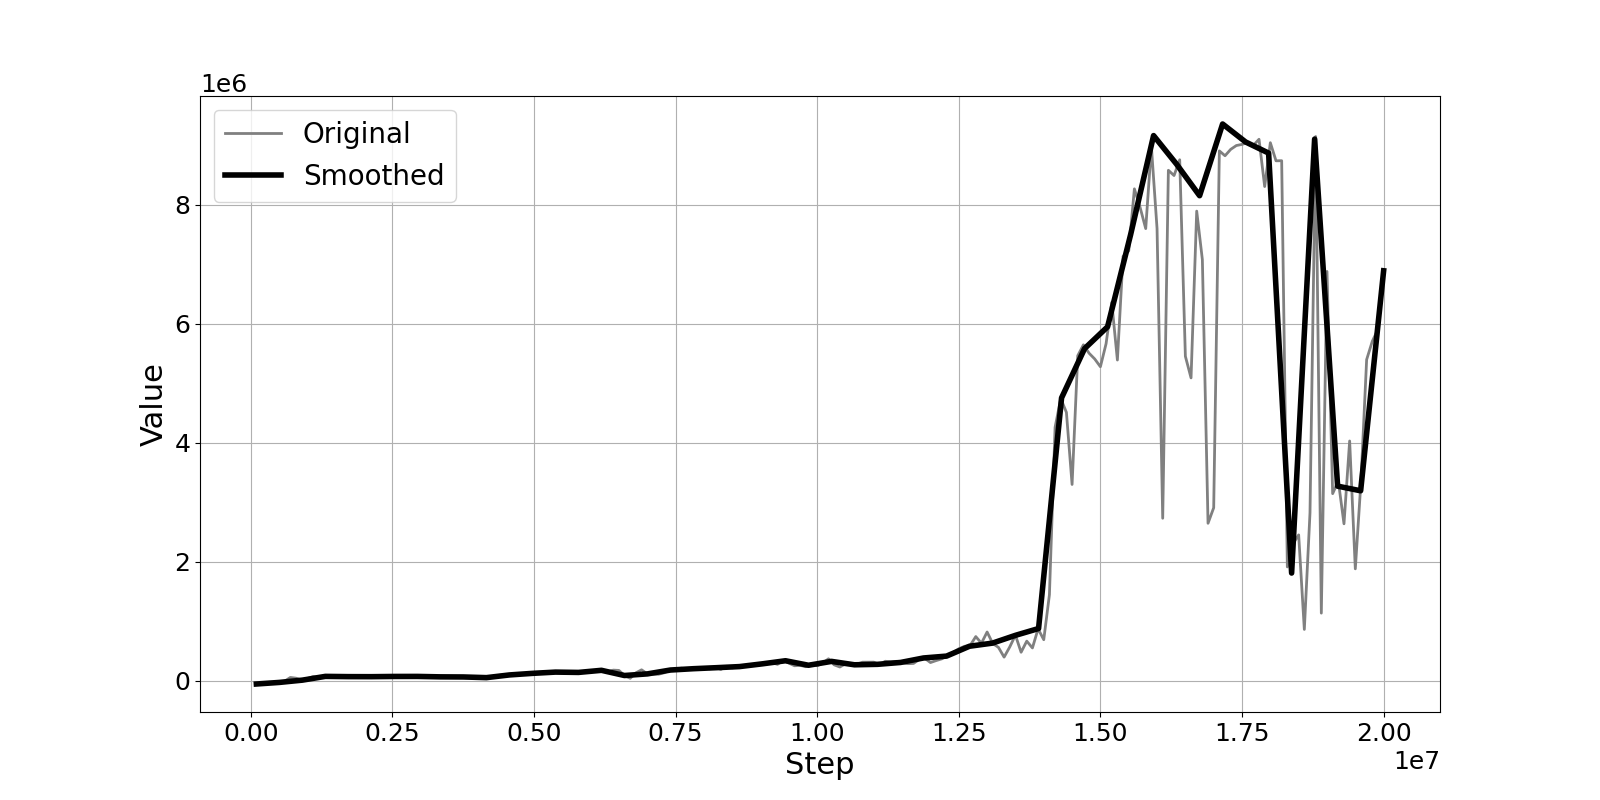
\includegraphics[width=1.1\textwidth]{figures/learning_curve/pendubot_learning_curve_redraw.png} % First image
    \caption{Pendubot learning curve}
    \label{fig:pendubot_learning_curve_ideal}
\end{figure}

Experiments on the acrobot during the ideal simulation phase were based on Design C, with \( l_1 \) set to 0.2m and \( l_2 \) to 0.3m. As depicted in Figure \ref{fig:acrobot_learning_curve_ideal}, the acrobot underwent a total of 3e7 timesteps of learning. Initially, the learning curve exhibited relatively steady growth up until 1.9e7 timesteps. Afterwards, the learning curve began to increase drastically after that. By 3e7 timesteps, the learning curve had not yet reached stability. This learning of 3e7 timesteps delivered a working agent, but the behaviour was not stable. Consequently, we extended the learning period to 5e7 timesteps, using a warm start from the agent obtained at 3e7 timesteps, and observed that the learning curve began to stabilize around 4e7 timesteps. The resulting agent has a good result in ideal simulation.

\begin{figure}[H]
    \centering
    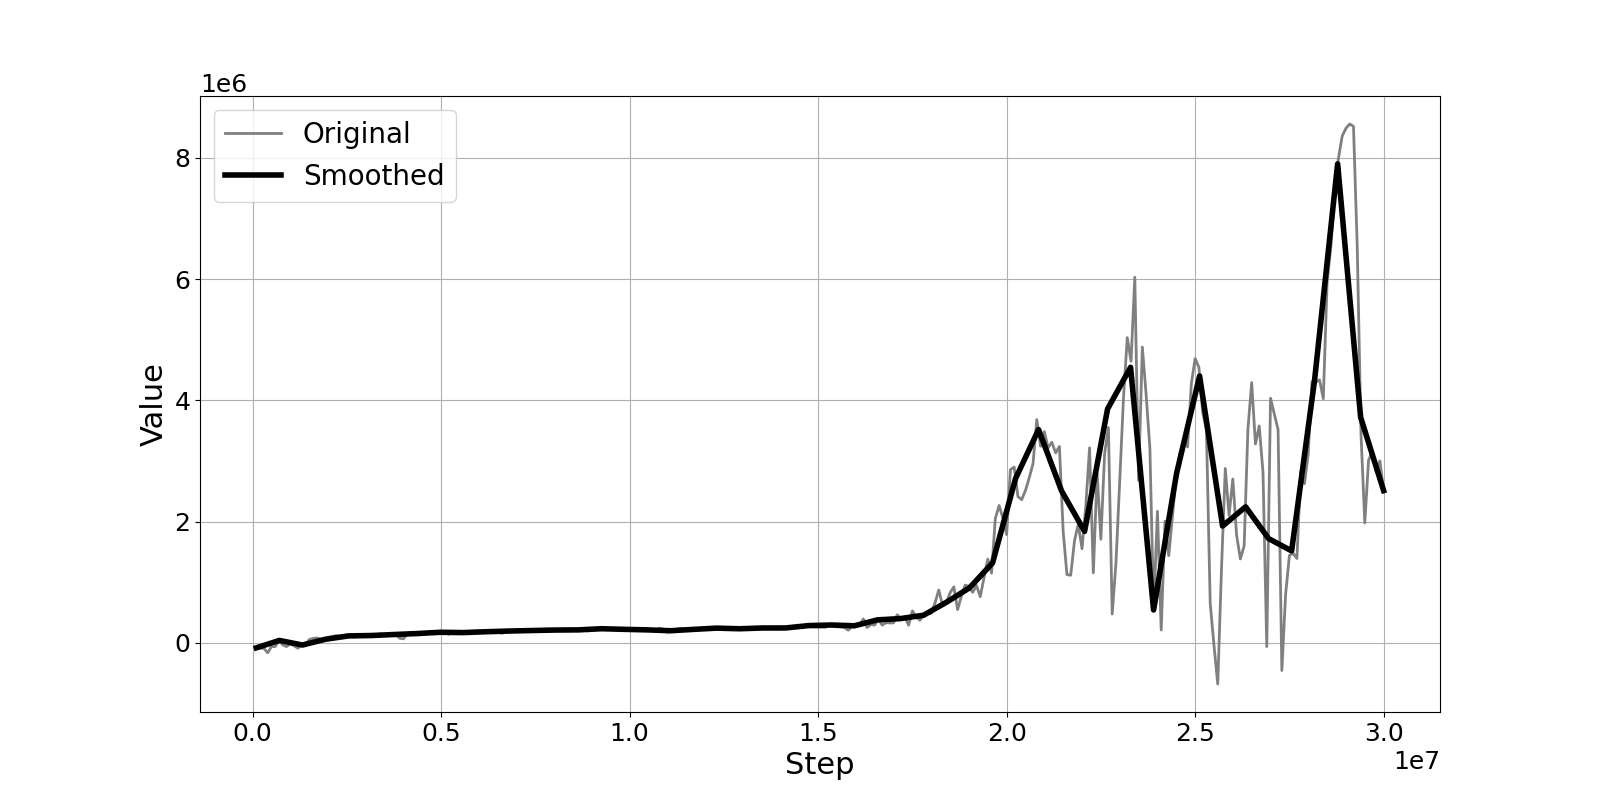
\includegraphics[width=1.1\textwidth]{figures/learning_curve/acrobot_learning_curve_redraw.png} % Second image
    \caption{Acrobot learning curve}
    \label{fig:acrobot_learning_curve_ideal}
\end{figure}

\section{Results in ideal simulation}
In this section, the ideal simulation results for the acrobot and pendubot are presented separately. Agents trained using the SAC algorithm are generally utilized during the swing-up stage, and the systems transition to the LQR controller when approaching the upright position. The primary criteria for success in both the swing-up and stabilization tasks involve swinging the double pendulum up to the upright position and maintaining stability for a prolonged period. Therefore, a simulation duration of 10 seconds is established. If the double pendulum fails to swing up or maintain stability within this timeframe, the trial is deemed unsuccessful.

\subsection{Pendubot simulation in ideal environment}
In the testing environment employed, also referred to as the ideal environment, disturbances such as friction and damping are excluded, with the focus placed solely on the effects of gravity, joint torque, and mechanical constraints. Zero initialization, as opposed to noisy initialization, is utilized, meaning the system commences from an initial state of \([0,0,0,0]^\text{T}\), indicating a start at zero position with zero velocity, and the swing-up is initiated using a control policy exclusively derived from SAC.

As depicted in Figure \ref{fig:ideal_simulation_pendubot}, the swing-up time is under 1 second, after which the state of the pendubot enters the Region of Attraction (ROA) for the LQR controller. The transition between the two controllers is seamless and effective, with the LQR controller subsequently maintaining the system's stability at the desired state. This demonstrates the effectiveness of the ROA method for LQR control takeover.

A significant highlight from this successful simulation is the impressively short swing-up time, despite having strict torque limit in place. However, a concerning feature observed from this simulation is the noisiness of the input control signal. The torque alternates signs rapidly, and the gradient of the torque tends to have a high absolute value.

\begin{figure}[H]
    \centering
    \fbox{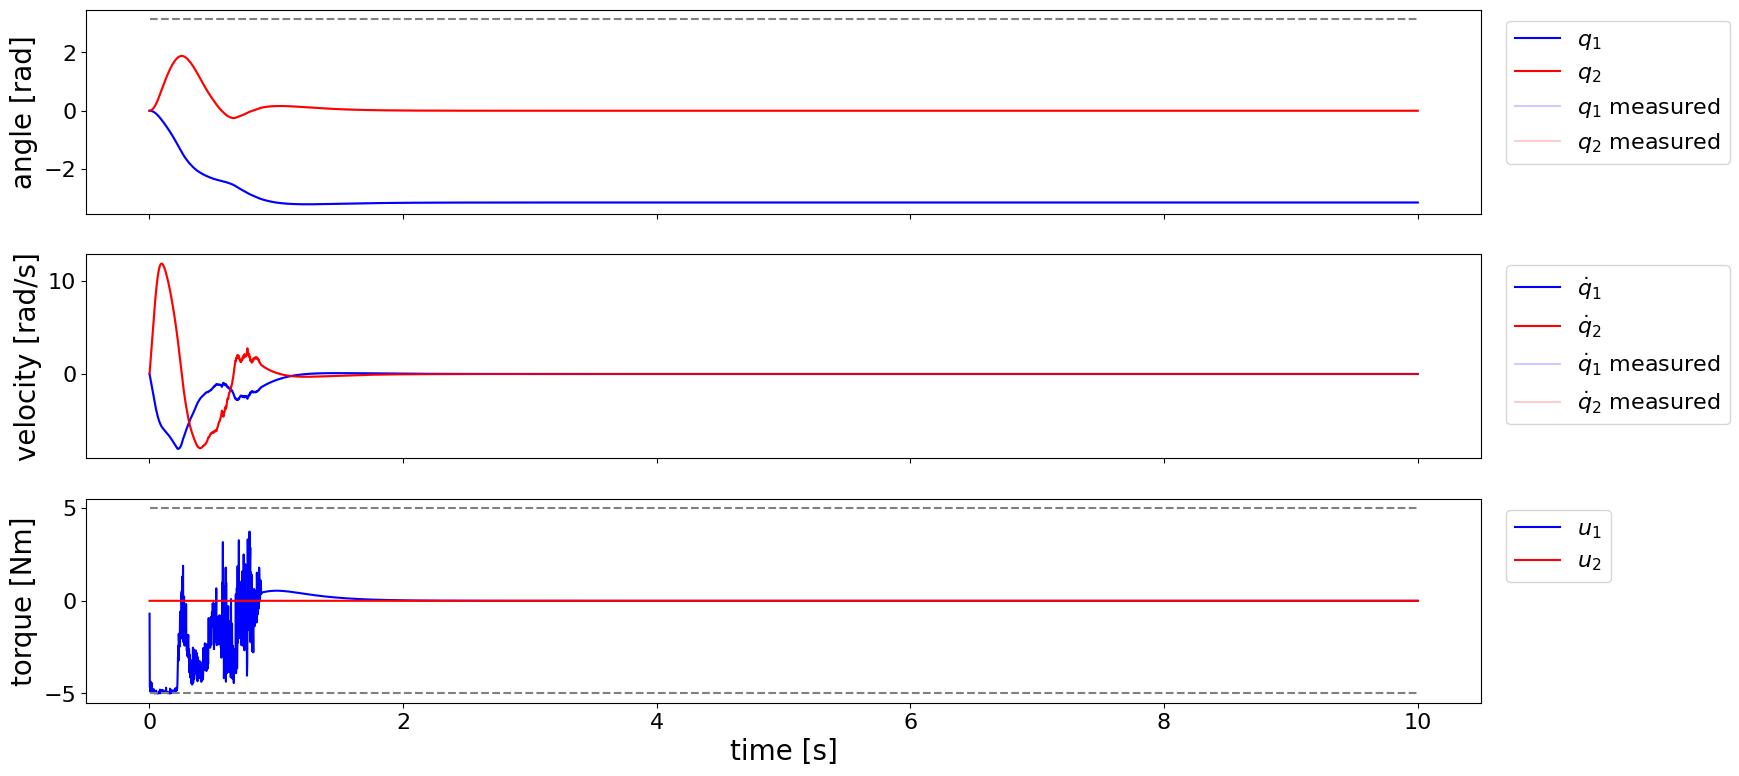
\includegraphics[width=0.9\textwidth]{figures/simulation_result/pendubot_unclipped.png}} % First image
    \caption{Pendubot result in ideal simulation }
    \label{fig:ideal_simulation_pendubot}
\end{figure}

\subsection{Acrobot simulation in ideal environment}

Just like the pendubot simulation, experiments on the acrobot setup are conducted in an ideal environment. The acrobot begins its swing from the downward position with zero velocity, aiming to stabilize around its highest point.

\begin{figure}[H]
    \centering
    \fbox{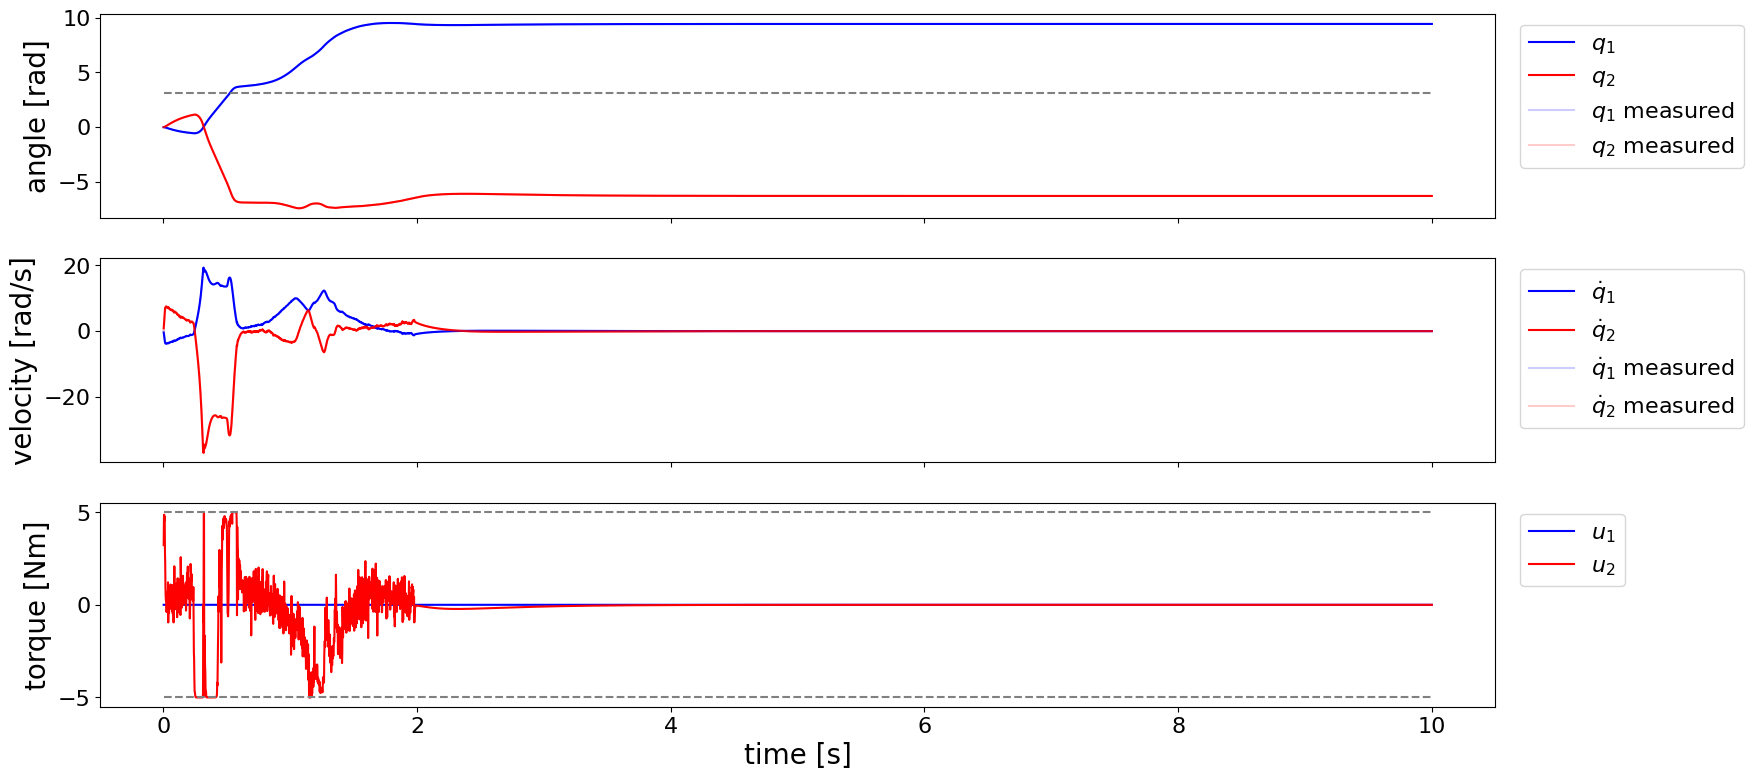
\includegraphics[width=0.9\textwidth]{figures/simulation_result/acrobot_unclipped.png}} % Second image
    \caption{Acrobot result in ideal simulation}
    \label{fig:ideal_simulation_acrobot}
\end{figure}

The accompanying image (Figure \ref{fig:ideal_simulation_acrobot}) depicts a successful swing-up and stabilization within a 10-second window. The swing-up process takes approximately 2 seconds before the LQR controller effectively takes over, maintaining stability around the target state for a prolonged time period.

In comparison to the pendubot's simulation curves, the swing-up time for the acrobot is longer. This aligns with the notion that controlling the acrobot is a more challenging task than the pendubot. A shared drawback observed in both simulations is the lack of torque smoothness. For the acrobot, the input torque exhibits several significant jumps from one torque limit to the other, which might cause difficulties when translating to real-world hardware control.

\subsection{Self stablizing behaviour on both pendubot and acrobot}
An unexpected outcome emerged during the testing of the swing-up and stabilization of the underactuated double pendulum system using only the RL-learned policy. It was observed that some agents not only entered the Region of Attraction (ROA) of the LQR controller as intended but also remained upright for an extended period without LQR assistance. This self-stabilizing behavior was noticeable in both the pendubot and acrobot configurations.

In the pendubot setup, self-stabilization was more frequently observed. With a sufficient number of training timesteps (typically around 2e7), agents tasked with swing-up maneuvers in the pendubot configuration were highly likely to achieve self-stabilization at the upright position. As depicted in Figure \ref{fig:pendubot_self_stabilization}, the stabilization by the RL-learned policy is less smooth compared to that achieved by the LQR-based stabilizer. The torque fluctuations have an amplitude of approximately 1.5 Nm, and there are minor fluctuations in position and velocity.

Self-stabilization behavior has been observed in the acrobot setup as well. However, no consistent pattern has yet been identified as to the specific conditions under which the training yields a self-stabilizing agent. Fortunately, the same agent discussed in Section 4.3.2 exhibited a degree of self-stabilization, which is depicted in Figure \ref{fig:acrobot_self_stabilization}. In the absence of a LQR controller, the RL-based controller was compelled to devise its own stabilization strategy. As illustrated in the graph, a relatively stable period commences at approximately 4 seconds, during which the system state exhibits prolonged fluctuations around the upright position. This occurs as the controller continuously corrects any deviation from the desired state. The stabilization provided by the RL-based controller is also less smooth than that of the LQR-based controller.

\begin{figure}[H]
    \centering
    \fbox{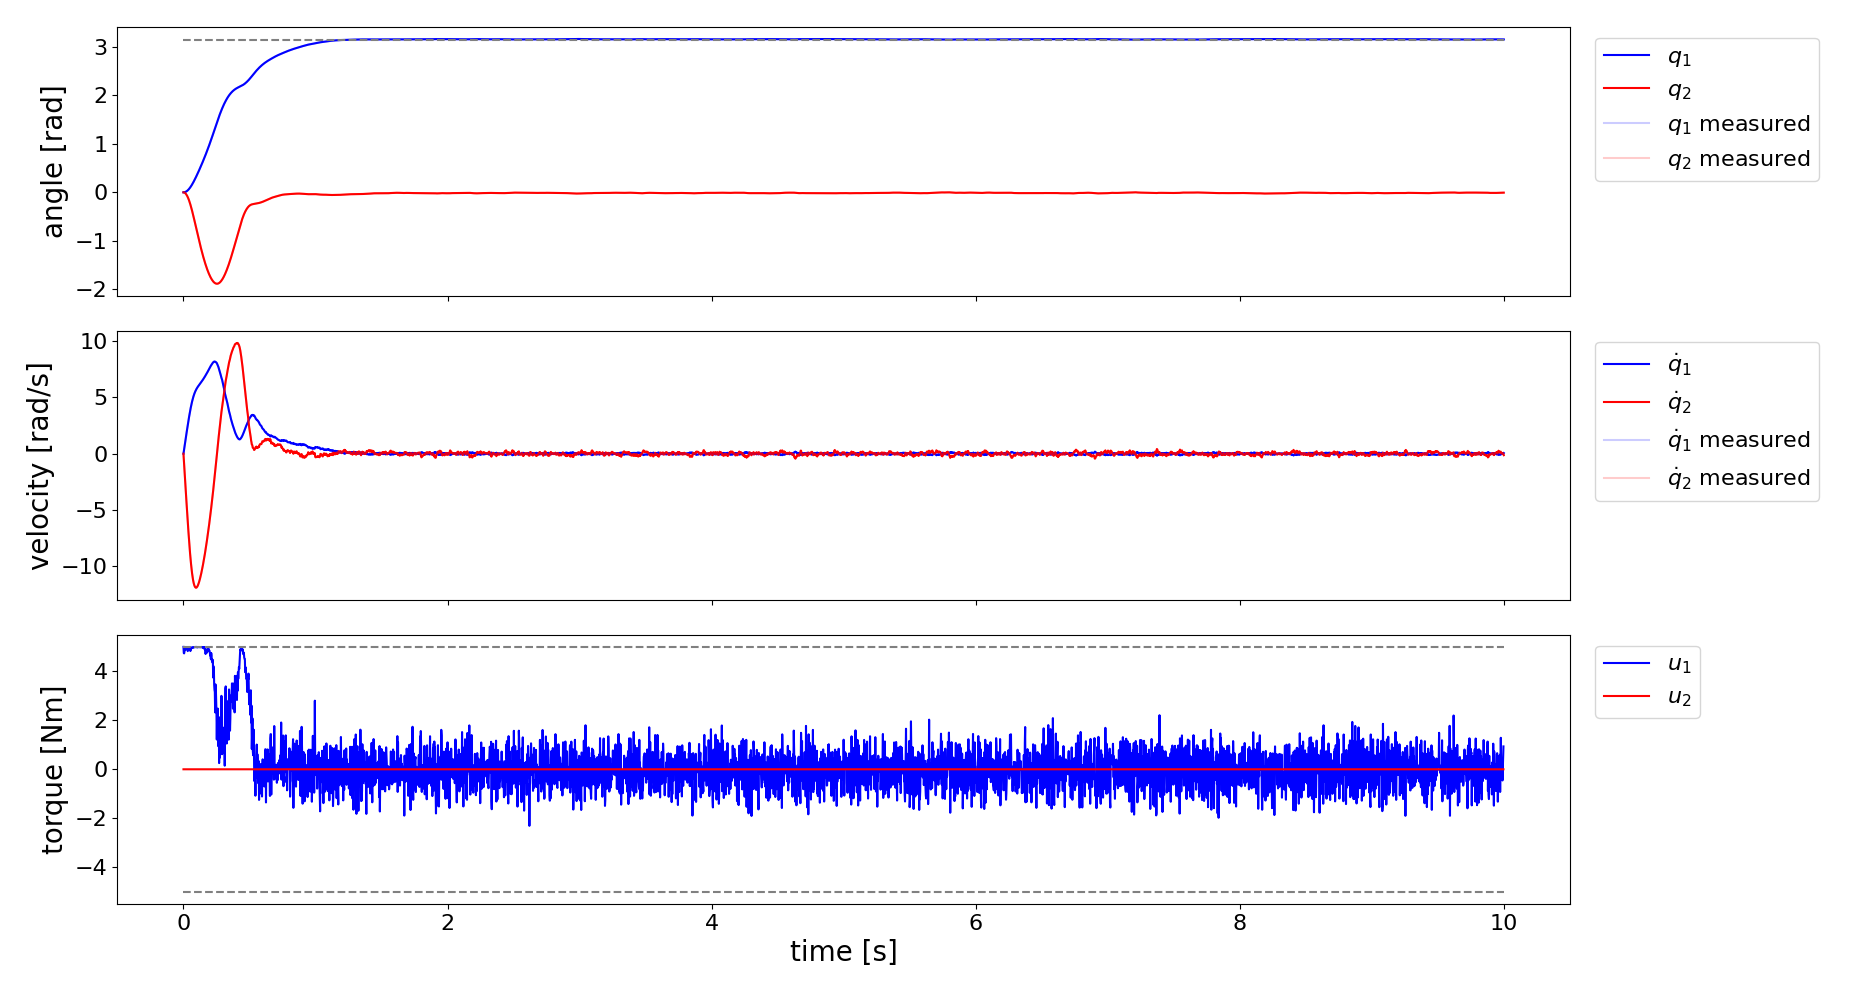
\includegraphics[width=0.9\textwidth]{figures/simulation_result/pendubot_self_stabilization.png}} % First image
    \caption{Self stabilization of pendubot in ideal simulation}
    \label{fig:pendubot_self_stabilization}
\end{figure}

\begin{figure}[H]
    \centering
    \fbox{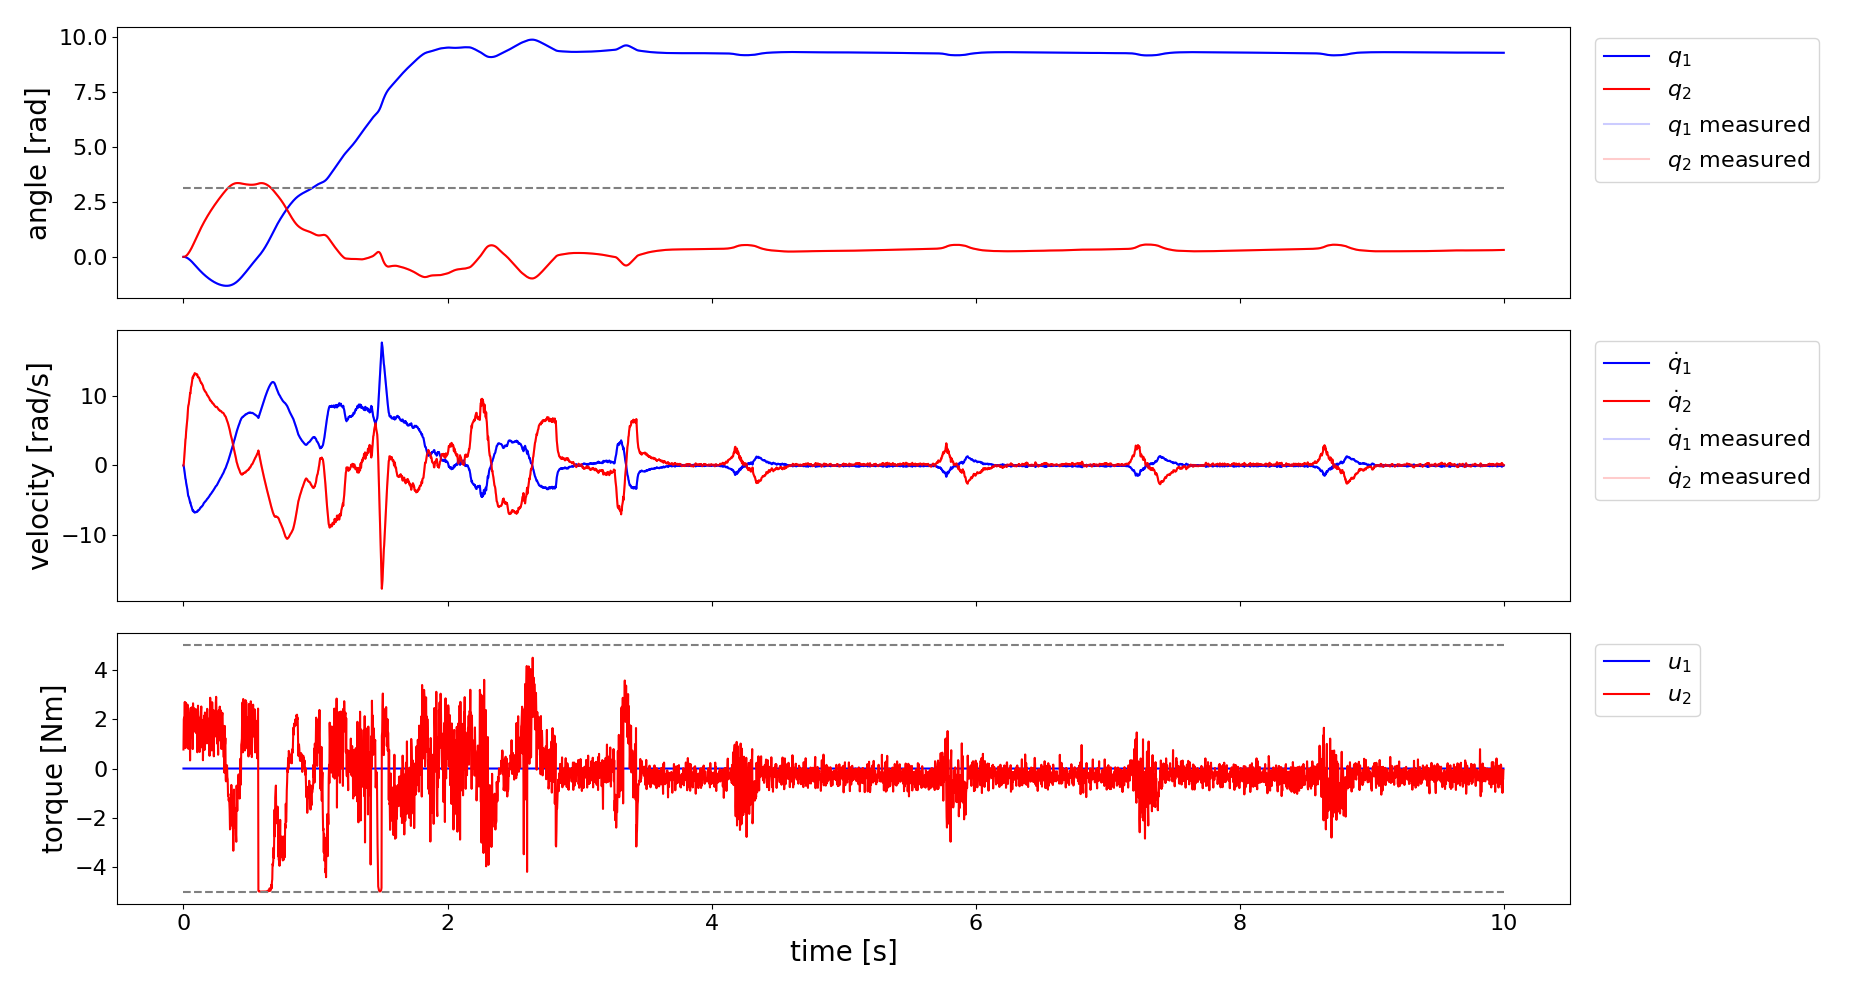
\includegraphics[width=0.9\textwidth]{figures/simulation_result/acrobot_self_stabilization.png}} % First image
    \caption{Self stabilization of acrobot in ideal simulation}
    \label{fig:acrobot_self_stabilization}
\end{figure}

\cleardoublepage
